\documentclass{article}
\usepackage[left=1in, right=1in, top=1in]{geometry}
\usepackage[utf8]{inputenc}
\usepackage{amsmath, amssymb, stmaryrd, bm, color}
\usepackage{hyperref}
\usepackage{graphicx}
\graphicspath{ {figures/} }
\usepackage{makecell}
\usepackage{float}
\usepackage{xcolor}

\title{Ellipsoidal Approximations}
\author{Tiancheng Ge}
\date{April 2019}

\begin{document}

\maketitle
\section*{Introduction}
This report summarizes the ellipsoidal approximation algorithms used in the ellipsoidal CInvS report. All the method calculates the approximation using closed form, instead of using descend based optimization methods. Note that some of the algorithms can find the optimal approximation, and some of them are just a approximation that runs fast.

\tableofcontents

\section{Representing ellipsoids}
Let $E \in \mathbb{R}^{n\times n}$ be a positive definite $n$-dimensional matrix, and $c \in \mathbb{R}^{n}$ be a $n$-dimensional vector. Then, an $n$-dimensional ellipsoidal set centered at $c$ can be represented as 
$$
\{x \in \mathbb{R}^{n} | (x-c)^T E (x-c)\leq 1 \}
$$

This $E$-$c$ notation will be used throughout this document and the code implementation on github
\href{https://github.com/getc1995/ellipsoidal_cinv.git}{https://github.com/getc1995/ellipsoidal\_cinv.git}

Denote $Q = E^{-1}$, and $Q = \Lambda \Lambda^T$. Then another way to get an ellipsoid is doing an affine transformation on a unit ball, and then translate it by a offset vector $c$.
%  is the singular value decomposition of $Q$. $Q$ and $F$ are both positive definite matrices, and $F$ is a diagonal matrix. 
\begin{align*}
&\{x \in \mathbb{R}^{n}\; |\; (x-c)^T E (x-c)\leq 1 \}\\
=& \{ \Lambda y + c \;|\; y \in \mathbb{R}^{n}, \|y\|_2 \leq 1 \}\\
=& \{ U F^{1/2}y + c \;|\; y \in \mathbb{R}^{n}, \|y\|_2 \leq 1 \}
\end{align*}
where $Q = \Lambda \Lambda^T = U F U^T$, and $U F U^T$ is a singular value decomposition of $Q$. $F$ is a diagonal matrix, and each diagonal entry of $F^{\frac{1}{2}}$ represents the length of the principal semi-axis of the ellipsoid. $U$ is a rotation matrix, and each row of it is a unit vector that represents the new direction of the coordinate after the rotation operation. While $E$-$c$ representation is easy to calculate the pre set, another notation that uses the $\Lambda$ and $c$ is easy to calculate the post set.

The volume of ellipsoid $V$ is 
\begin{align*}
&\;\;V\\
= &\;\; C(n) \det(F^{\frac{1}{2}})\\
= &\;\; C(n) \sqrt{\det(Q)}\\
= &\;\; C(n) \frac{1}{\sqrt{\det(E)}}\\
\end{align*}
and $C(n)$ is a constant that depends on the dimensionality, for example, $C(2) = 2\pi$. For all the ellipsoidal approximations in this report, we try to find the ellipsoid with maximum or minimum volume. If the problem is convex, then the optimal ellipsoidal approximation is affine invariant.

\section{Approximation algorithms}

\subsection{Intersection of two concentric ellipsoids, inner approximation}
\begin{table}[H]
\centering
\begin{tabular}{ccc}
\includegraphics[width=0.3\textwidth]{intersect_concentric_ia/1.pdf} & 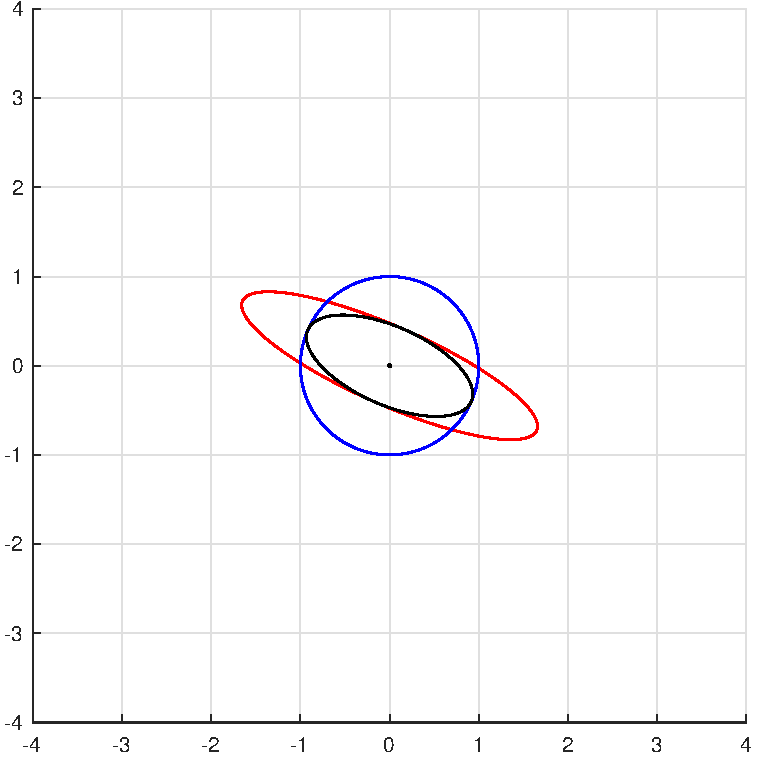
\includegraphics[width=0.3\textwidth]{intersect_concentric_ia/2.pdf} & 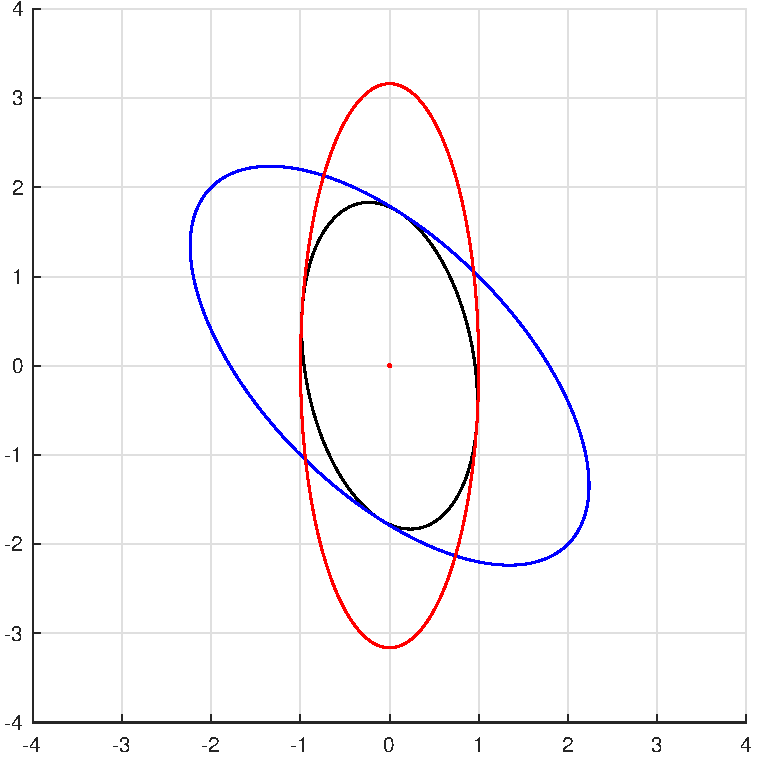
\includegraphics[width=0.3\textwidth]{intersect_concentric_ia/3.pdf}\\
Original & \makecell{Apply an affine transformation \\such that one of the ellipsoid \\becomes a unit sphere} & Affine transformation back
\end{tabular}
%\caption{Table of figures}
\label{intersect_concentric_ia}
\end{table}
    
Assuming we have two concentric ellipsoids. To find the optimal inner approximation, we can apply an affine transformation to both ellipsoids together, such that one of them becomes a unit sphere. 

The maximum inscribed ellipsoid of the intersection is the maximum ellipsoid whose principal axes are aligned with the red ellipsoid.

This method can give the optimal approximation for the intersection of two ellipsoids. However, for the intersection of three or more ellipsoids, applying this method on two ellipsoids at a time wouldn't give the optimal inner approximation.

The implementation is in \texttt{ellipsoidal\_approximation/intersect\_concentric\_ia.m}

\subsection{Union of two concentric ellipsoids, outer approximation}
\begin{table}[H]
	\centering
	\begin{tabular}{ccc}
		\includegraphics[width=0.3\textwidth]{union_concentric_oa/1.pdf} & 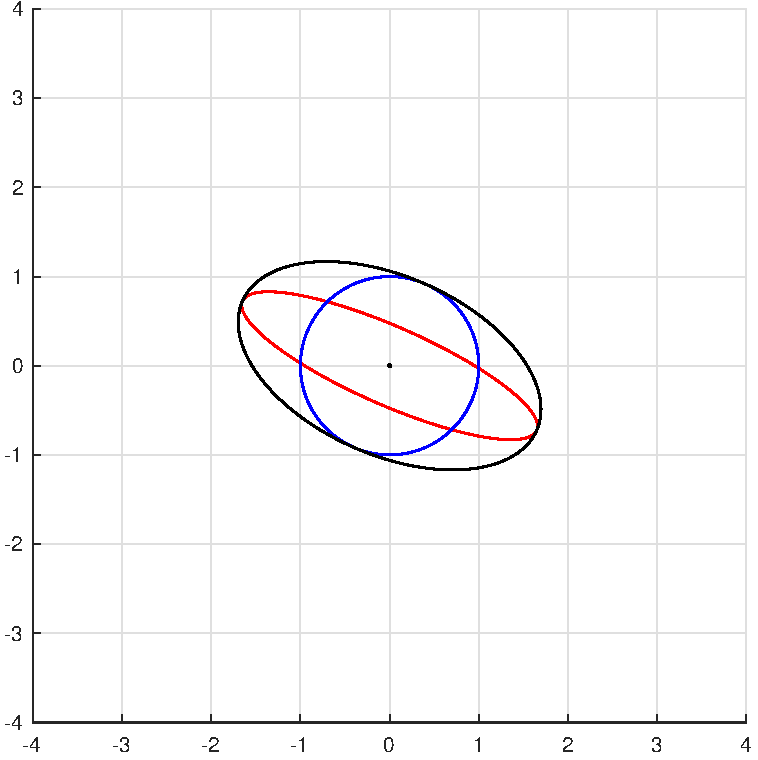
\includegraphics[width=0.3\textwidth]{union_concentric_oa/2.pdf} & 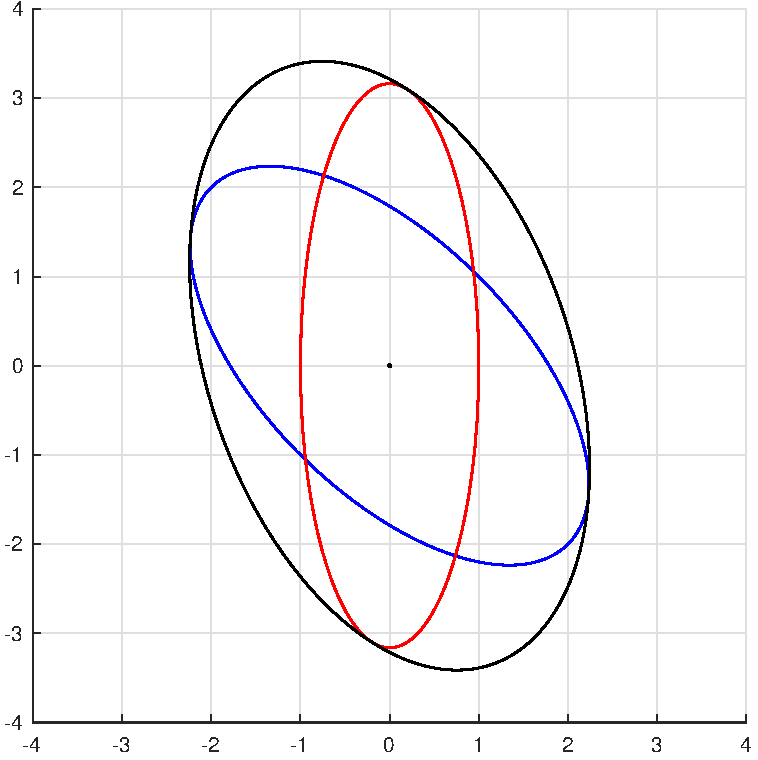
\includegraphics[width=0.3\textwidth]{union_concentric_oa/3.pdf}\\
		Original & \makecell{Apply an affine transformation \\such that one of the ellipsoid \\becomes a unit sphere} & Affine transformation back
	\end{tabular}
	%\caption{Table of figures}
	\label{union_concentric_oa}
\end{table}

The idea of the method is the same as finding inner approximation for intersection.

This method can give the optimal approximation for the union of two ellipsoids. However, for the union of three or more ellipsoids, applying this method on two ellipsoids at a time wouldn't give the optimal outer approximation.

The implementation is in \texttt{ellipsoidal\_approximation/union\_concentric\_oa.m}

\subsection{Intersection of an ellipsoid and a symmetric polytope, inner approximation}

A symmetric polytope centered at origin can be decomposed into pairs of parallel hyperplanes. To find an approximation (not an optimal one) for the intersection of an ellipsoid and a symmetric polytope, we can find the intersection of the ellipsoid and halfspace pairs one by one.

The following is the procedure for finding the optimal inner approximation of the intersection of an ellipsoid and two halfspaces.

\begin{table}[H]
	\centering
	\begin{tabular}{ccc}
		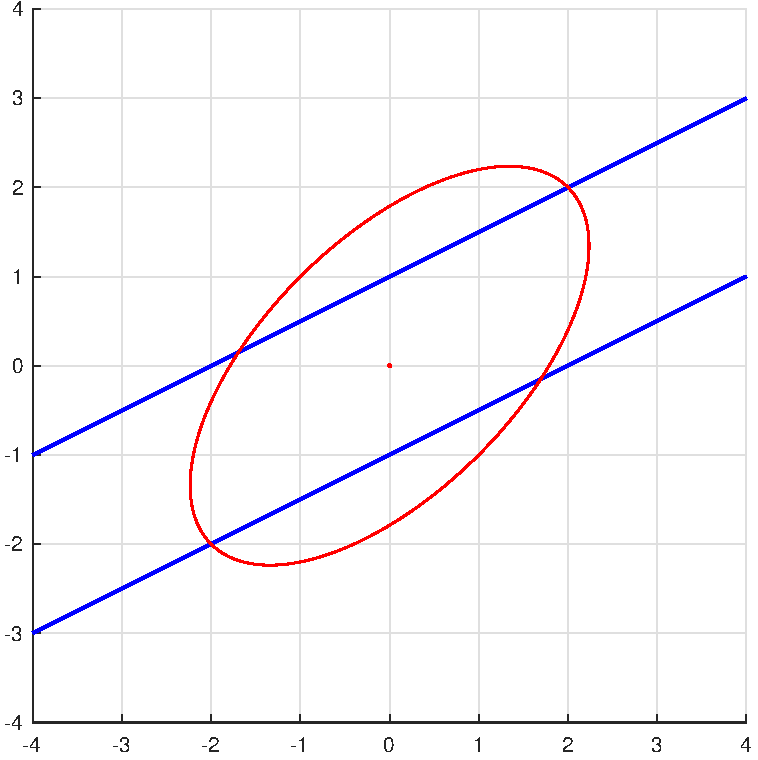
\includegraphics[width=0.3\textwidth]{polytope_intersect/1.pdf} & 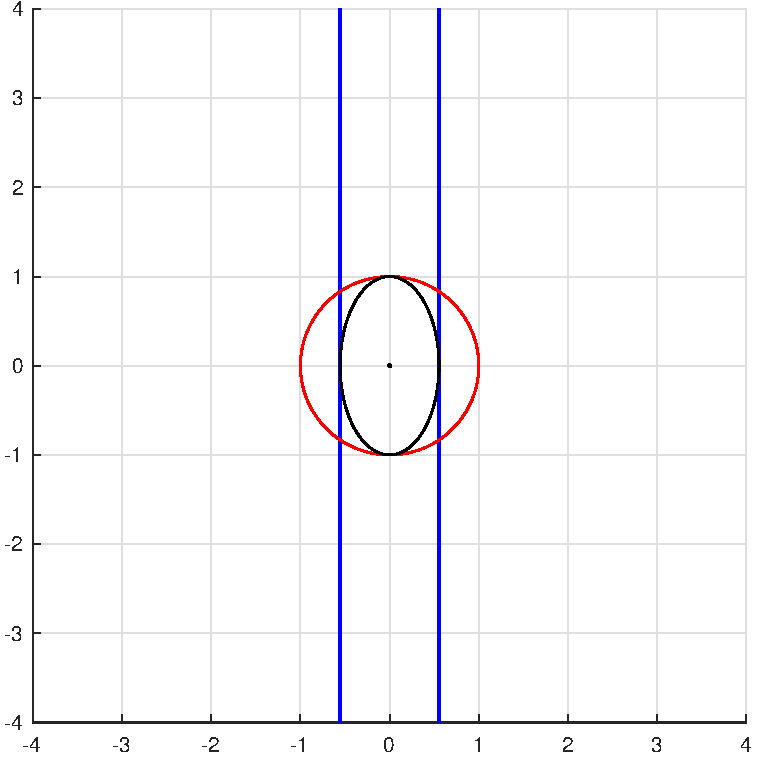
\includegraphics[width=0.3\textwidth]{polytope_intersect/2.pdf} & 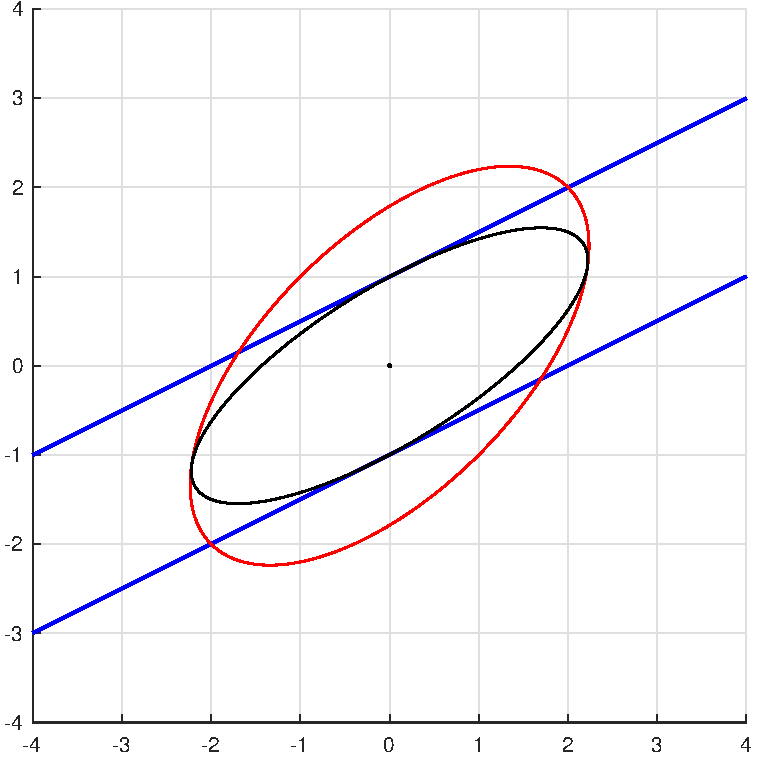
\includegraphics[width=0.3\textwidth]{polytope_intersect/3.pdf}\\
		Original & \makecell{Apply an affine transformation \\such that the ellipsoid \\becomes a unit sphere} & Affine transformation back
	\end{tabular}
	%\caption{Table of figures}
	\label{polytope_intersec1}
\end{table}

\begin{table}[H]
	\centering
	\begin{tabular}{ccc}
		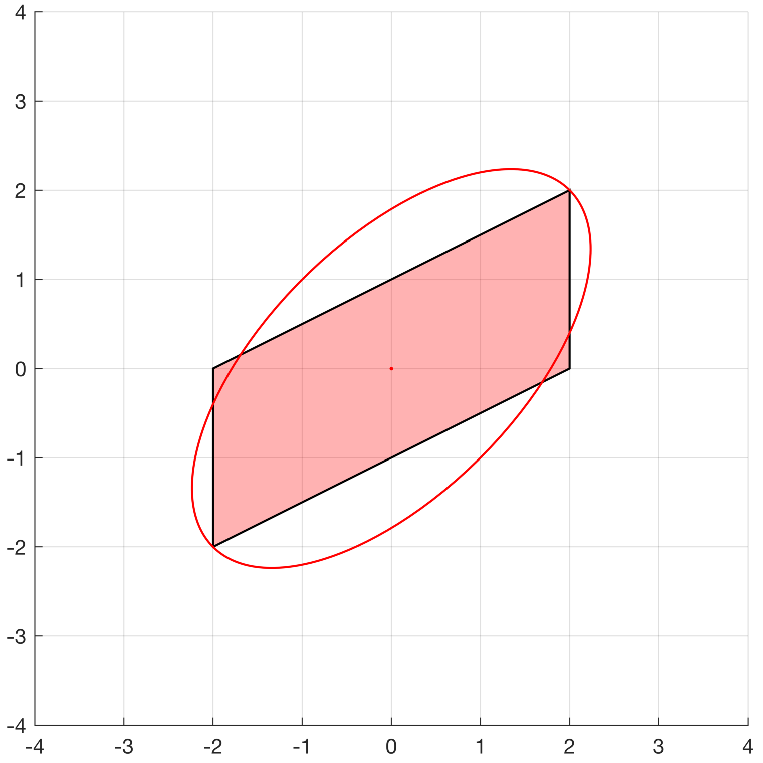
\includegraphics[width=0.3\textwidth]{polytope_intersect/4.pdf} & 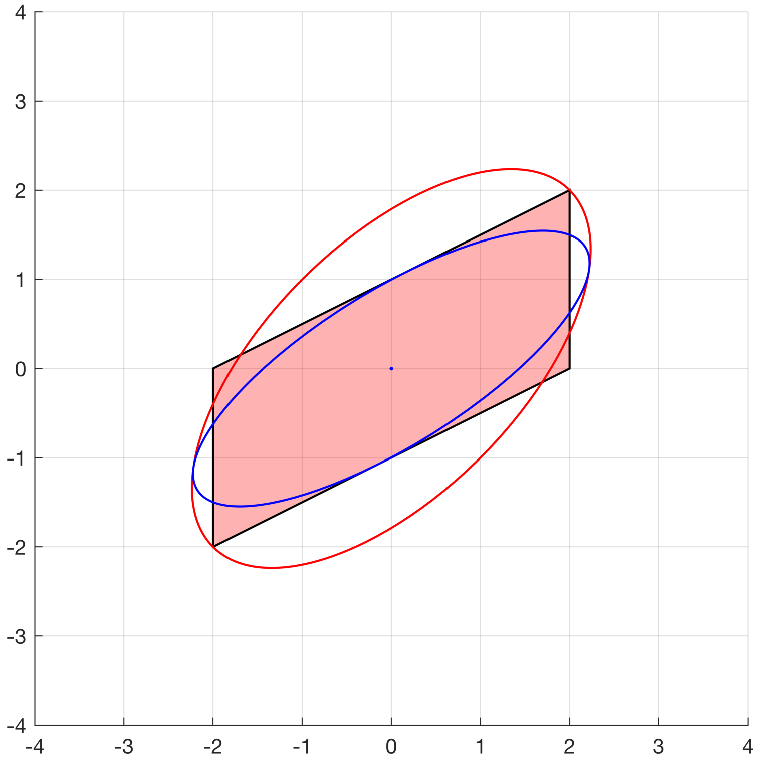
\includegraphics[width=0.3\textwidth]{polytope_intersect/5.pdf} & 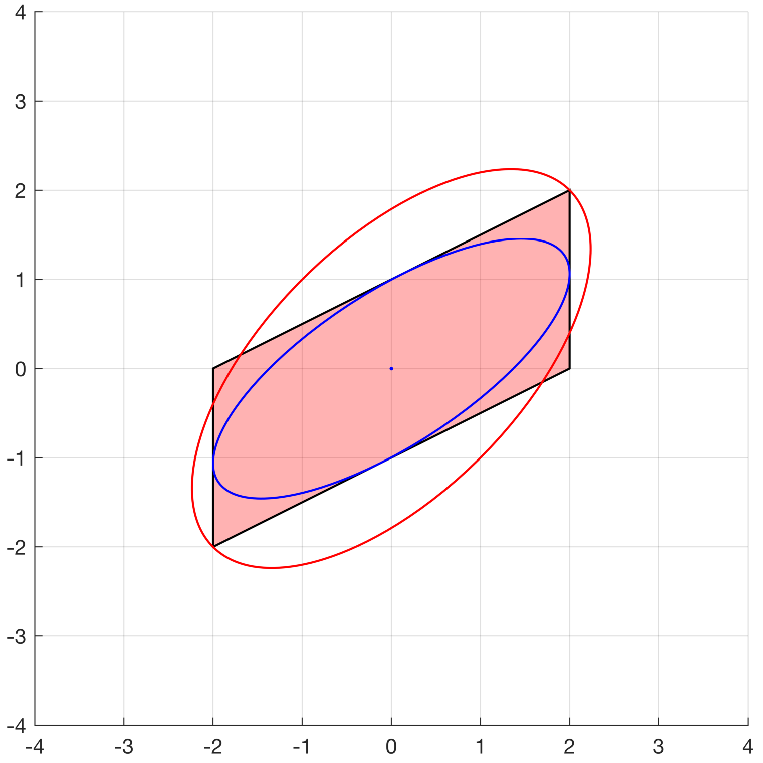
\includegraphics[width=0.3\textwidth]{polytope_intersect/6.pdf}\\
		Original & \makecell{Take the intersection with \\ one pair of halfspaces} & \makecell{Take the intersection with \\ other pair of halfspaces}
	\end{tabular}
	%\caption{Table of figures}
	\label{polytope_intersect2}
\end{table}

The above example happen to be the optimal inner approximation, because the inner approximated ellipsoid happened to have no intersection with the original ellipsoid, and it is the maximum inscribed ellipsoid of the polytope. However, if the optimal inner approximation have intersections with the original ellipsoid on the boundary, the approximation found by this procedure is not optimal.

Also, if the number of halfspace pairs is greater than the dimension of the ellipsoid, the approximation is not guaranteed to be optimal.

The implementation is in \texttt{ellipsoidal\_approximation/polytope\_intersect.m}

\subsection{Intersection of two offset unit balls, inner approximation}
\label{section_intersect_offset_unitball_ia}
\begin{figure}[h!]
	\centering
	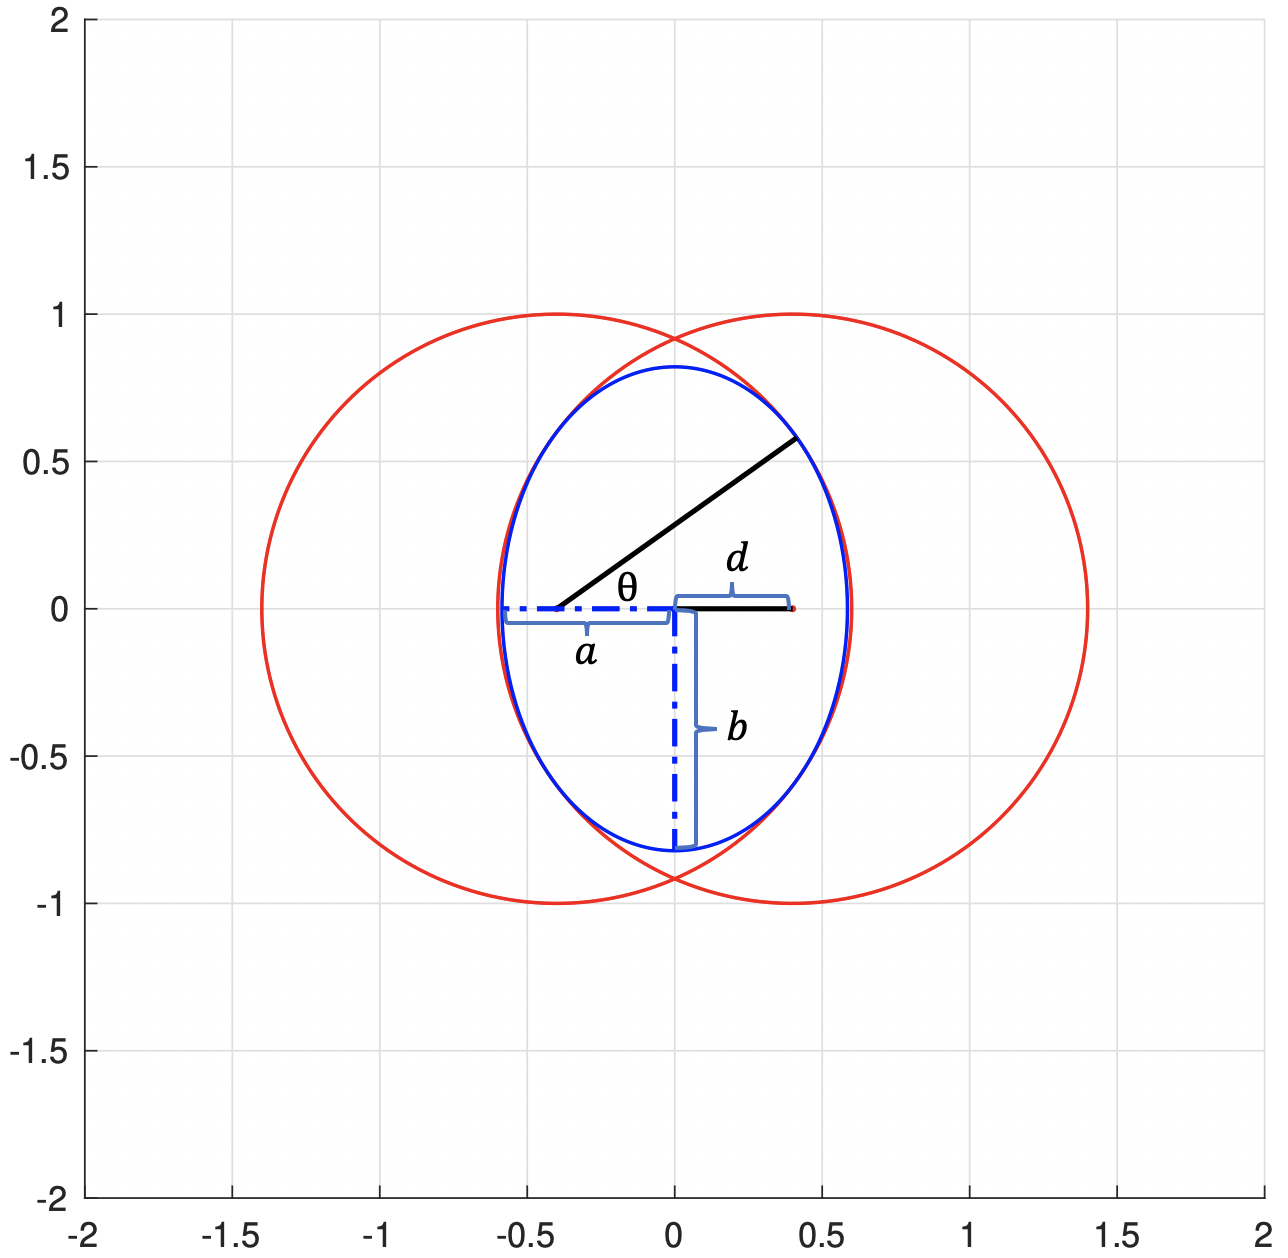
\includegraphics[width=0.6\linewidth]{intersect_offset_unitball_ia/1.png}
	\caption{The distance between two red unit circles is $2d$. The blue ellipse is maximum inscribed ellipse of the intersection of the two circles.}
	\label{intersect_offset_unitball_ia}
\end{figure}

The maximum inscribed ellipsoid must be centered at the origin due to the symmetric property. Say Figure \ref{intersect_offset_unitball_ia} is a cross-section of two $n$-dimensional ellipsoids. $a$ and $b$ are the length of two principal semi-axes of the inscribed ellipsoid. Due to the symmetrical property, the other principal semi-axes must have length $b$ as well. Therefore, the volume of the inscribed ellipsoid $V$ is proportional to $ab^{n-1}$.

Connect the center of the left circle and the intersection between left circle and the inscribed ellipse, whose coordinate is ($\cos\theta - d $, $\sin\theta$). Denote the angle of between the line and the horizontal axis to be $\theta$. Utilizing geometry properties 

\begin{enumerate}
\item intersection ($\cos\theta - d $, $\sin\theta$) is on the boundary of ellipsoid.
\item the tangent plane at the intersection to the ellipse is the tangent plane to the circle as well, and therefore the tangent plane is perpendicular to the line.
\end{enumerate}
we can express $a$ and $b$ in terms of $\theta$, and volume $V$ becomes a function of $\theta$ and the dimension $n$.

\begin{align*}
a & = \sqrt{\frac{(1-d\cos\theta)(\cos\theta-d)}{\cos\theta}}\\
b & = \sqrt{1 - d\cos\theta}
\end{align*}

Fixing the dimension $n$ and take the derivative of $V$ with respect to $\theta$ and set it to zero, we have 
$$
\cos\theta = \frac{(n-1)d}{2n} + \sqrt{\frac{1}{n} + \left(\frac{n-1}{2n}d\right)^2}
$$

which is a closed-form solution that defines the maximum inscribed ellipsoid.

The implementation is in \texttt{ellipsoidal\_approximation/intersect\_offset\_unitball\_ia.m}

\subsection{Convex hull of two offset unit balls, outer approximation}
\begin{figure}[H]
	\centering
	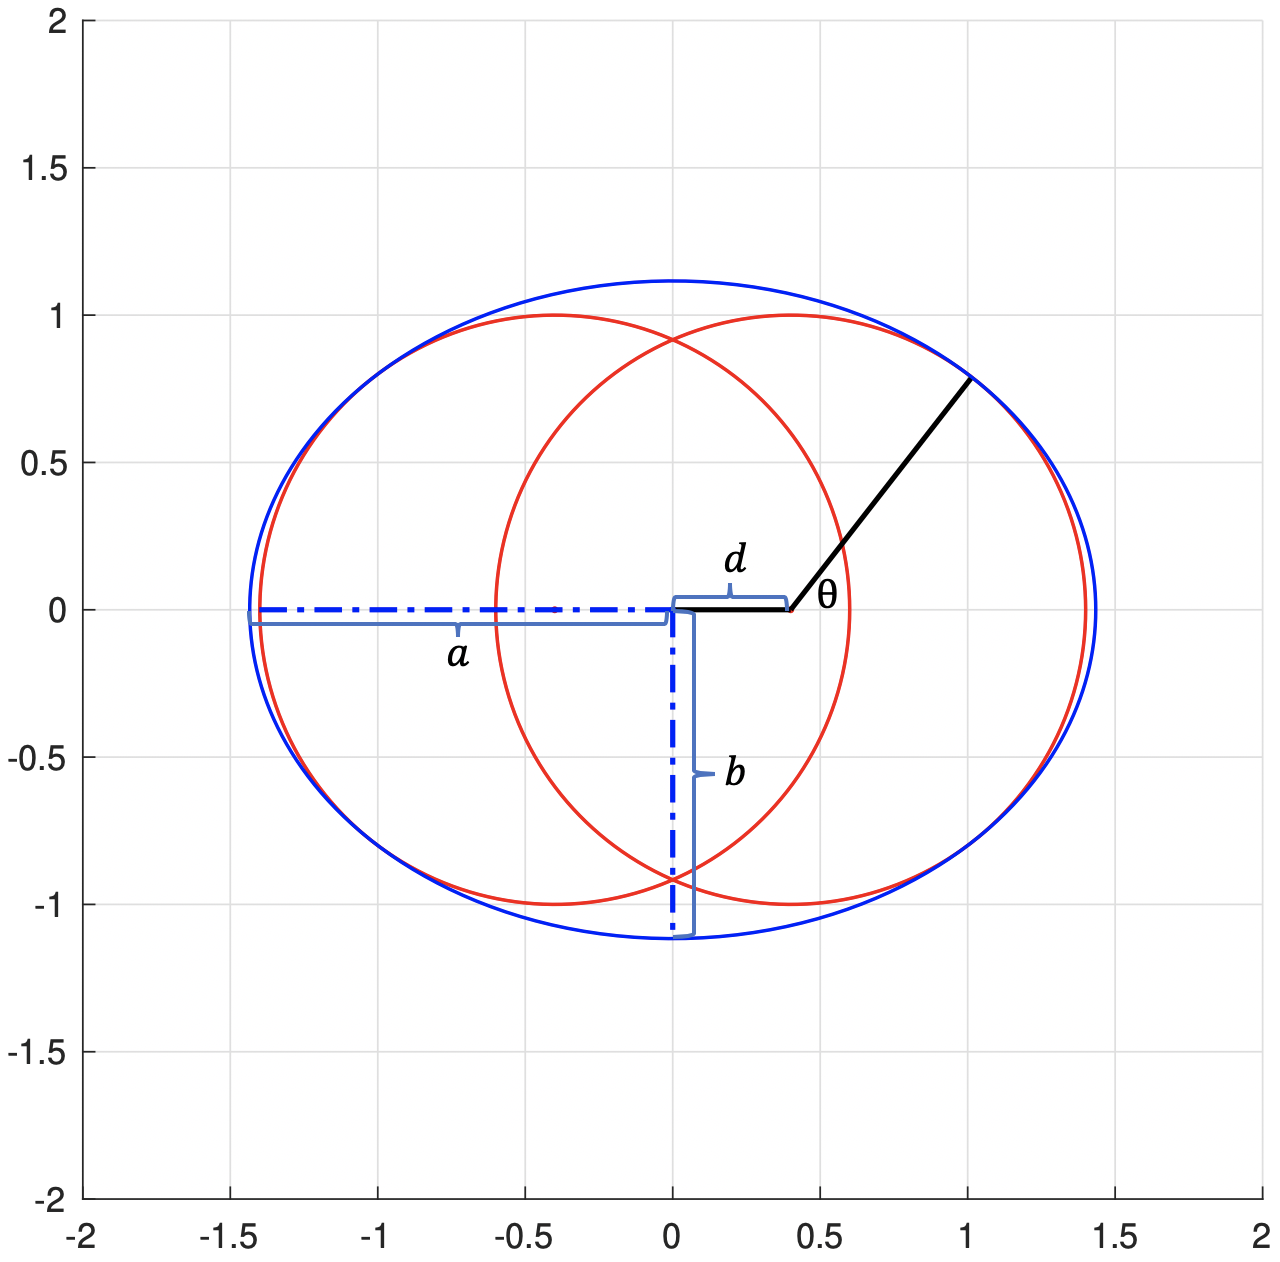
\includegraphics[width=0.6\linewidth]{union_offset_unitball_oa/1.png}
	\caption{The distance between two red unit circles is $2d$. The blue ellipse is minimum circumscribed ellipse of the convex hull of the two circles.}
	\label{union_offset_unitball_oa}
\end{figure}

Using the same idea in section \ref{section_intersect_offset_unitball_ia}, we have

\begin{align*}
\cos\theta &= -\frac{(n-1)d}{2n} + \sqrt{\frac{1}{n} + \left(\frac{n-1}{2n}d\right)^2}\\
a & = \sqrt{\frac{(1+d\cos\theta)(\cos\theta+d)}{\cos\theta}}\\
b & = \sqrt{1 + d\cos\theta}
\end{align*}

The implementation is in \texttt{ellipsoidal\_approximation/union\_offset\_unitball\_oa.m}

\subsection{Convex hull of two offset unit balls, inner approximation}
\begin{figure}[H]
	\centering
	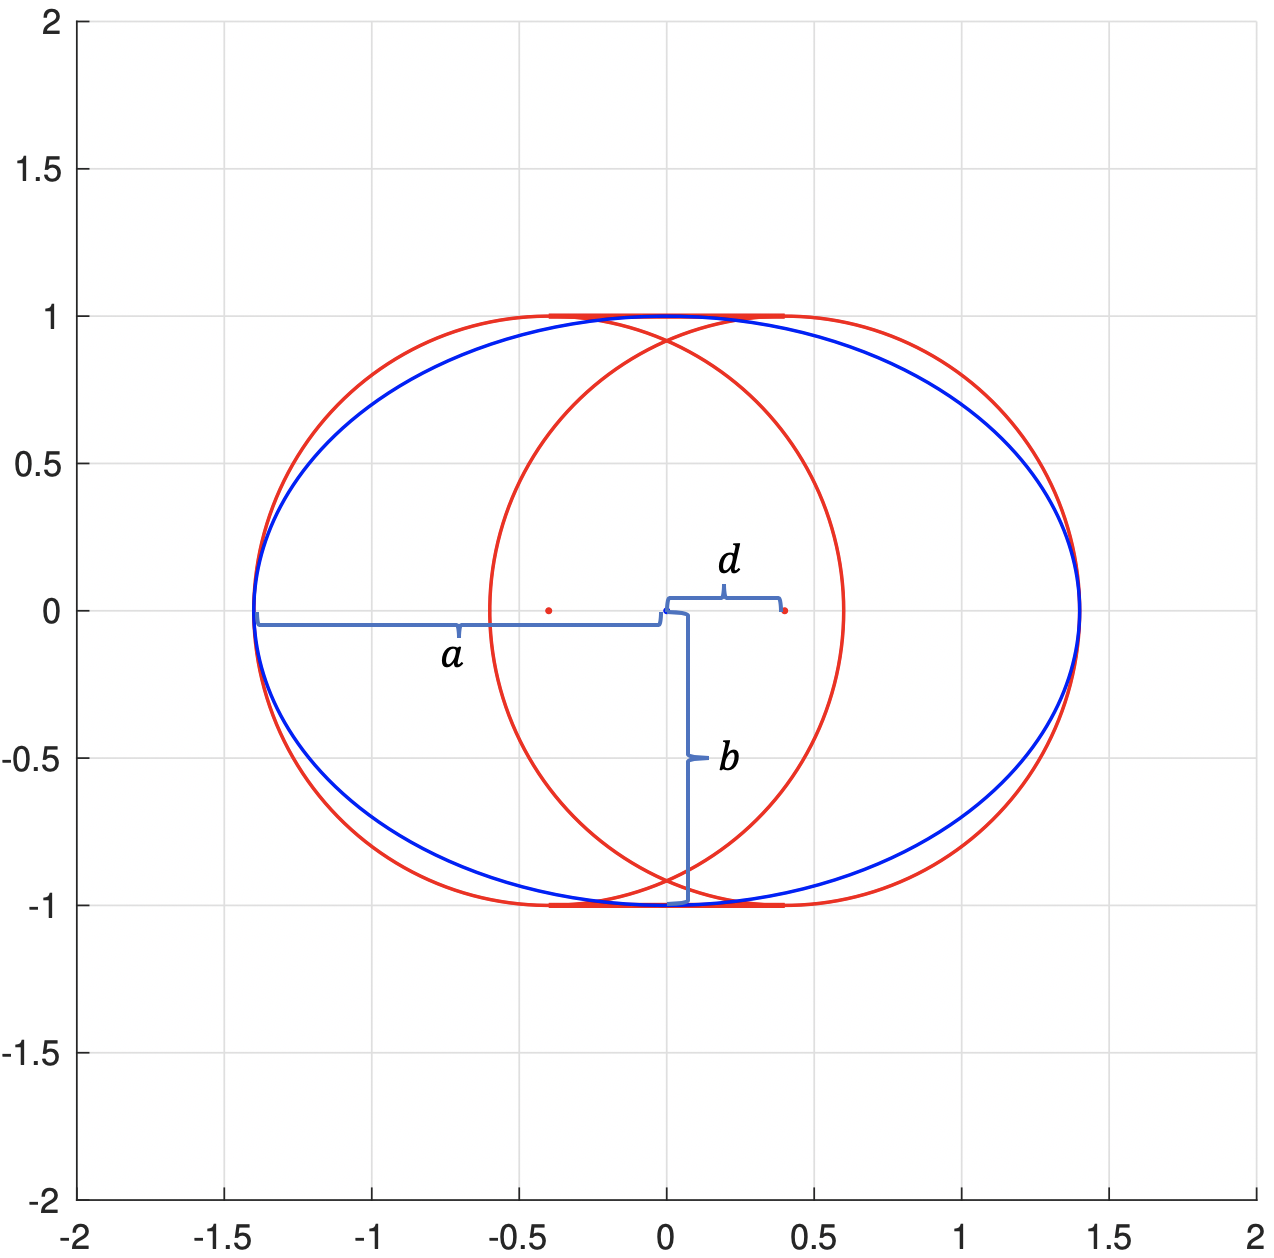
\includegraphics[width=0.5\linewidth]{union_offset_unitball_ia/1.png}
	\caption{The distance between two red unit circles is $2d$. The blue ellipse is maximum inscribed ellipse of the convex hull of the two circles. It is straightforward that $a=1+d$ and $b = 1$, due to the symmetrical property.}
	\label{union_offset_unitball_ia}
\end{figure}
The implementation is in \texttt{ellipsoidal\_approximation/union\_offset\_unitball\_ia.m}

\subsection{Minkowski difference of an ellipsoid and a parallelotope, inner approximation}
\label{intersect_offset_ia}
\begin{table}[h!]
	\centering
	\begin{tabular}{cc}
		\includegraphics[width=0.3\textwidth]{intersect_offset_ia/1.pdf} & \includegraphics[width=0.3\textwidth]{intersect_offset_ia/2.pdf} \\
		\makecell{Ellipsoid and parallelotope. \\ The two arrows are the disturbance \\ vectors that form the parallelotope.}& \makecell{Red ellipsoids are obtained by \\ shifting the blue ellipsoid to each \\ vertex of the parallelotope.\\ The Minkowski difference is \\the intersection of red ellipsoids.} 
	\end{tabular}
	%\caption{Table of figures}
	\label{intersect_offset_ia1}
\end{table}
The Minkowski difference of a convex set and a closed polytope can be found in the following way: For each vertex of the polytope, shift the convex set to that vertex. Then the intersection of all the shifted convex sets is the Minkowski difference.

For a parallelotope, its number of vertices is $2^n$, where $n$ is the dimension of the parallelotope. However, it is possible to utilize the symmetrical property of parallelotopes to reduce the computational complexity from depending on $n$ exponentially to polynomially.

An $n$ dimensional parallelotope can be defined by $n$ linearly independent vectors $v_1, \dots, v_n$, and can be represented as 
$$
\{ c_1 v_1 + \dots + c_n v_n  \;\; | \;\; c_1,  \dots,  c_n \in [-1, 1], v_1,  \dots,  v_n \in \mathbb{R}^n\}
$$

To calculate the Minkowski difference, we can compress the ellipsoid in each $v_i$ direction, that is to calculate the intersection of the original ellipsoid offset by $2v_i$. Notice that this algorithm still works even in the case of degenerated parallelotope (one or more vector $v_i$ is $\mathbf{0}$).

\begin{table}[h!]
	\centering
	\begin{tabular}{ccc}
		\includegraphics[width=0.3\textwidth]{intersect_offset_ia/3.pdf} & 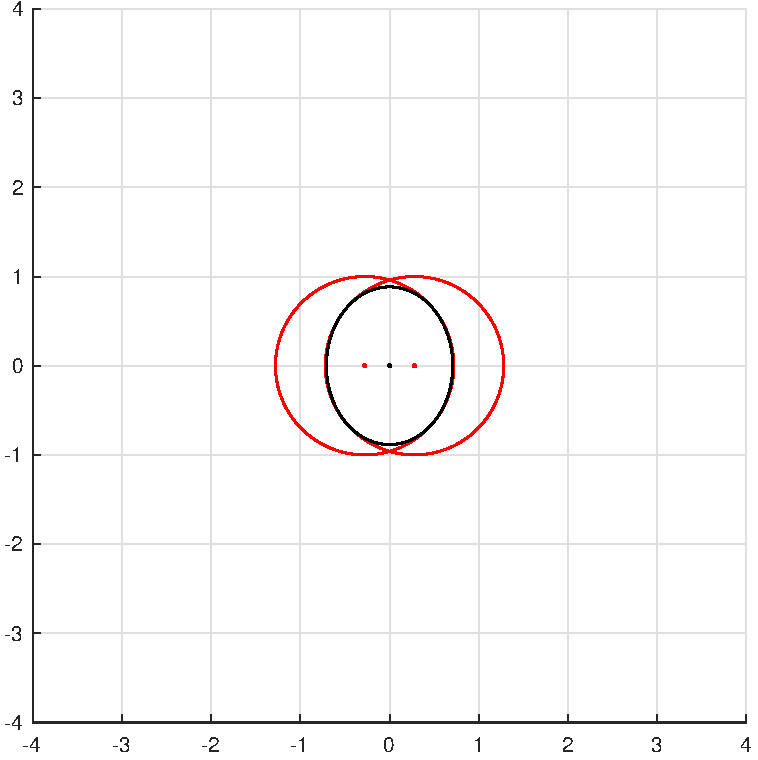
\includegraphics[width=0.3\textwidth]{intersect_offset_ia/4.pdf} & 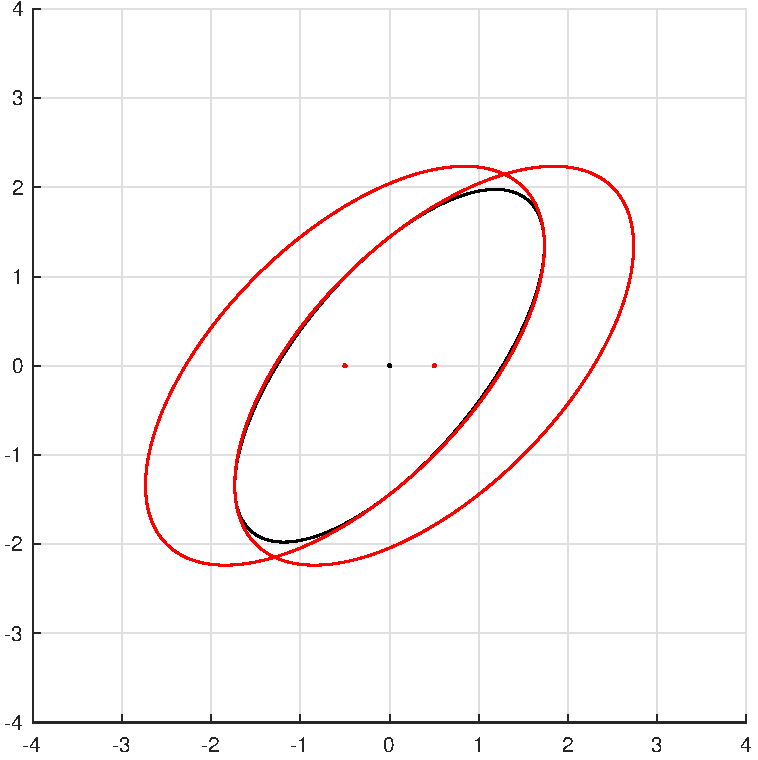
\includegraphics[width=0.3\textwidth]{intersect_offset_ia/5.pdf}\\
		Offset by $2v_1$ & \makecell{Apply an affine transformation \\such that the ellipsoids \\become unit spheres} & Affine transformation back \\
		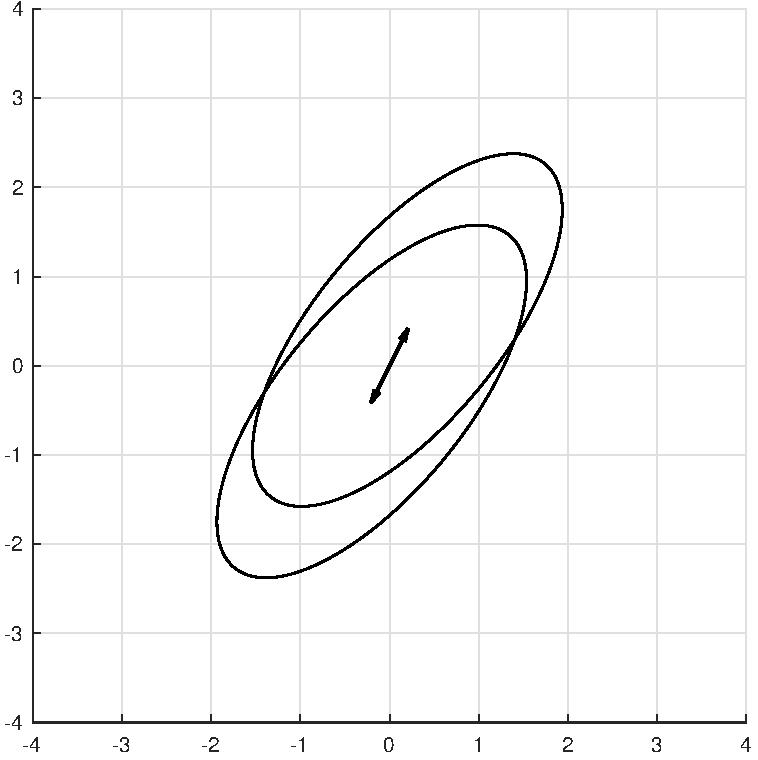
\includegraphics[width=0.3\textwidth]{intersect_offset_ia/6.pdf} & 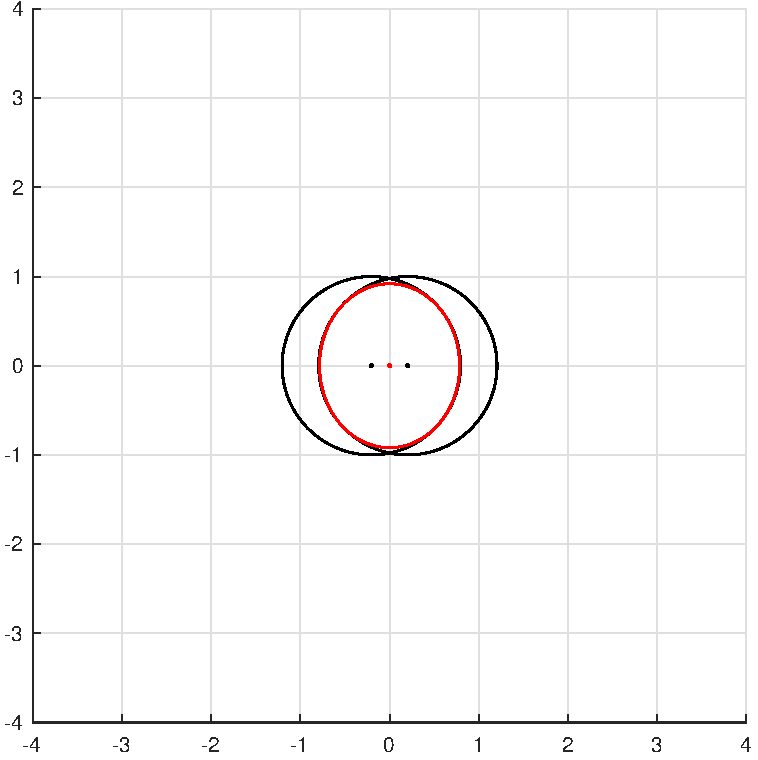
\includegraphics[width=0.3\textwidth]{intersect_offset_ia/7.pdf} & 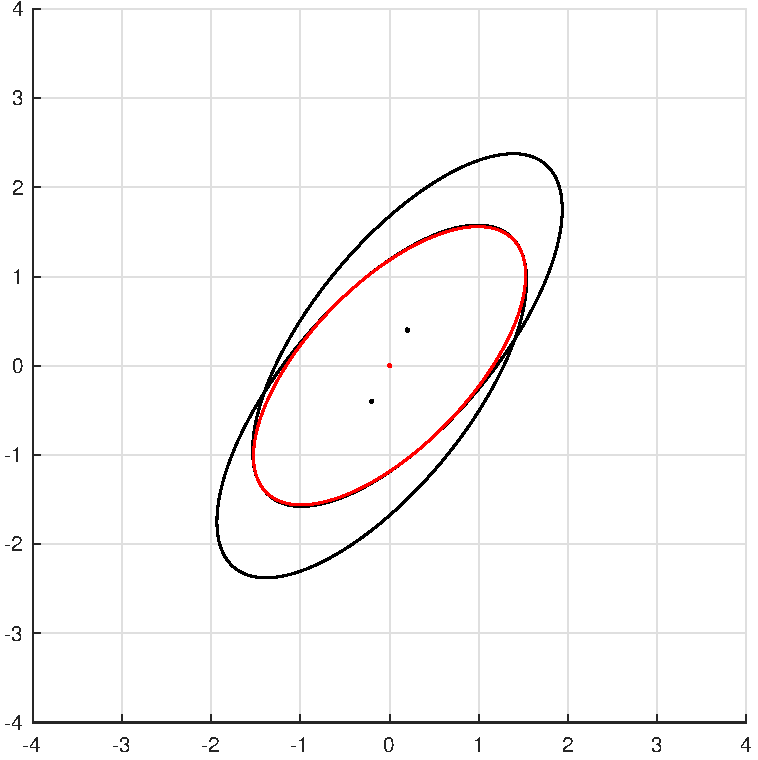
\includegraphics[width=0.3\textwidth]{intersect_offset_ia/8.pdf}\\
		Offset by $2v_2$ & \makecell{Apply an affine transformation \\such that the ellipsoids \\become unit spheres} & Affine transformation back
	\end{tabular}
	%\caption{Table of figures}
	\label{intersect_offset_ia2}
\end{table}


\begin{figure}[H]
	\centering
	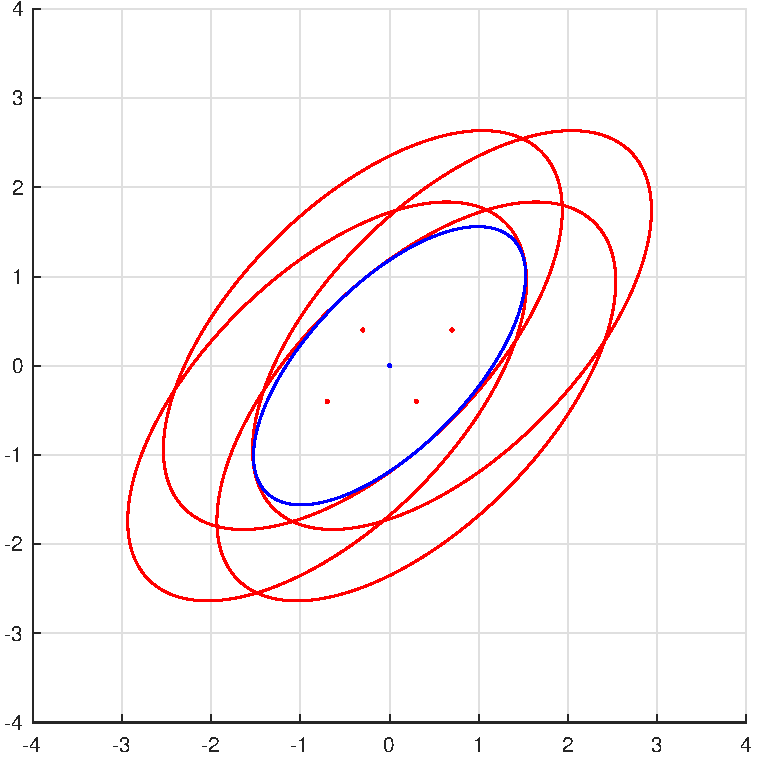
\includegraphics[width=0.3\linewidth]{intersect_offset_ia/9.pdf}
	\caption{The blue ellipsoid is an inscribed ellipsoid of the intersection of the red ellipsoid, calculated by the procedure above, and is an inner approximation of the Minkowski difference.}
	\label{intersect_offset_ia3}
\end{figure}

\textcolor{red}{TODO: prove that this algorithm gives the maximum inner approximation. }

The implementation is in \texttt{ellipsoidal\_approximation/intersect\_offset\_ia.m}


\subsection{Minkowski sum of an ellipsoid and a parallelotope, outer approximation}
Using the same idea in section \ref{intersect_offset_ia}. Here instead of compressing along each direction, we do ``stretching'', i.e., calculate the outer approximation of the convex hull of the two offset ellipsoids.

\begin{table}[h!]
	\centering
	\begin{tabular}{ccc}
		\includegraphics[width=0.3\textwidth]{union_offset_oa/1.pdf} & \includegraphics[width=0.3\textwidth]{union_offset_oa/2.pdf} & 
		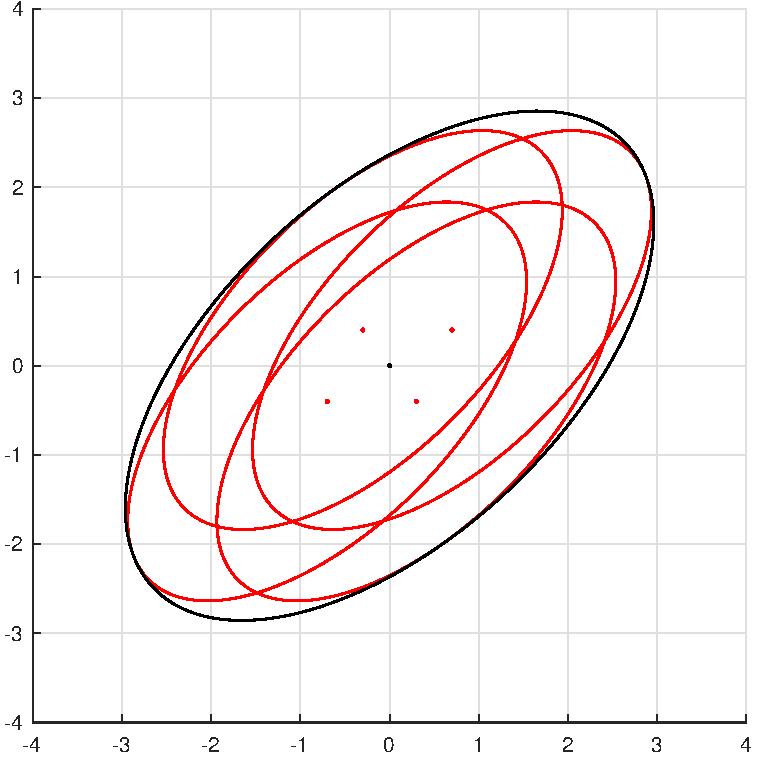
\includegraphics[width=0.3\textwidth]{union_offset_oa/9.pdf}\\
		\makecell{Ellipsoid and parallelotope. \\ The two arrows are the control \\ vectors that form the parallelotopic \\ control set.}& \makecell{Red ellipsoids are obtained by \\ shifting the blue ellipsoid to each \\ vertex of the parallelotope.\\ The Minkowski sum is \\the convex hull of red ellipsoids.} & \makecell{The black ellipsoid is the\\ calculated outer approximation.}
	\end{tabular}
	%\caption{Table of figures}
	\label{union_offset_oa1}
\end{table}

\begin{table}[H]
	\centering
	\begin{tabular}{ccc}
		\includegraphics[width=0.3\textwidth]{union_offset_oa/3.pdf} & 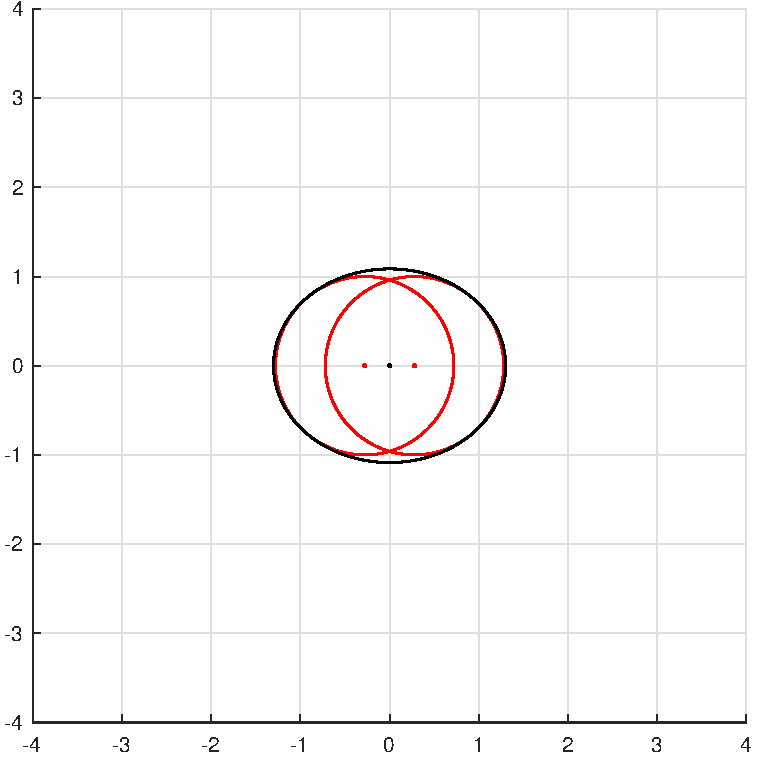
\includegraphics[width=0.3\textwidth]{union_offset_oa/4.pdf} & 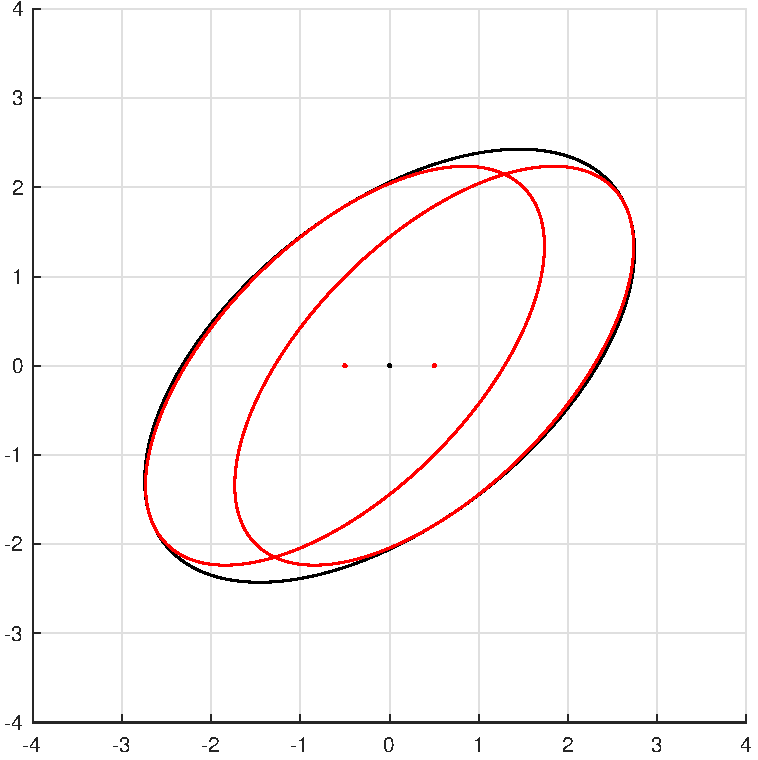
\includegraphics[width=0.3\textwidth]{union_offset_oa/5.pdf}\\
		Offset by $2v_1$ & \makecell{Apply an affine transformation \\such that the ellipsoids \\become unit spheres} & Affine transformation back \\
		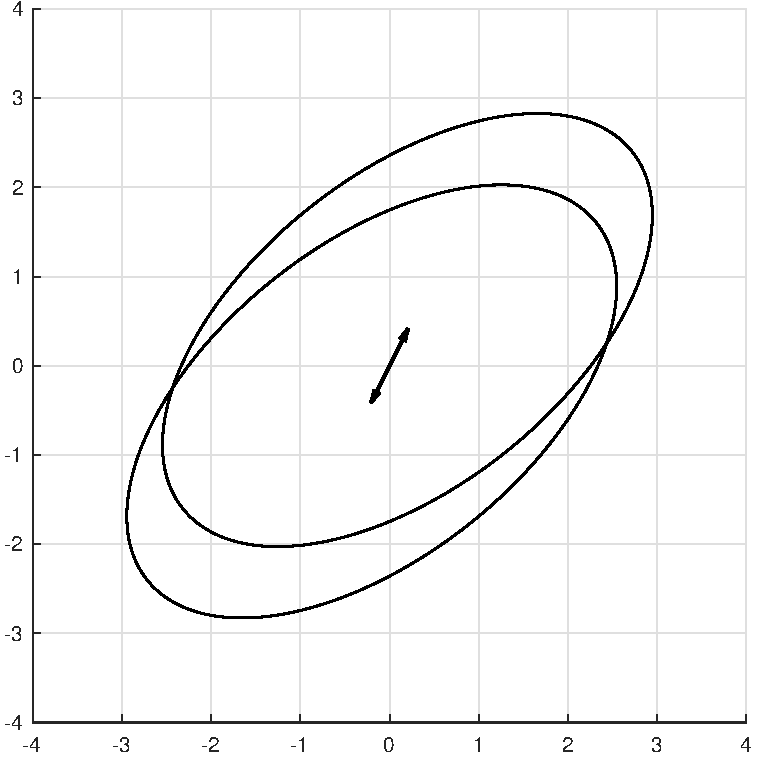
\includegraphics[width=0.3\textwidth]{union_offset_oa/6.pdf} & 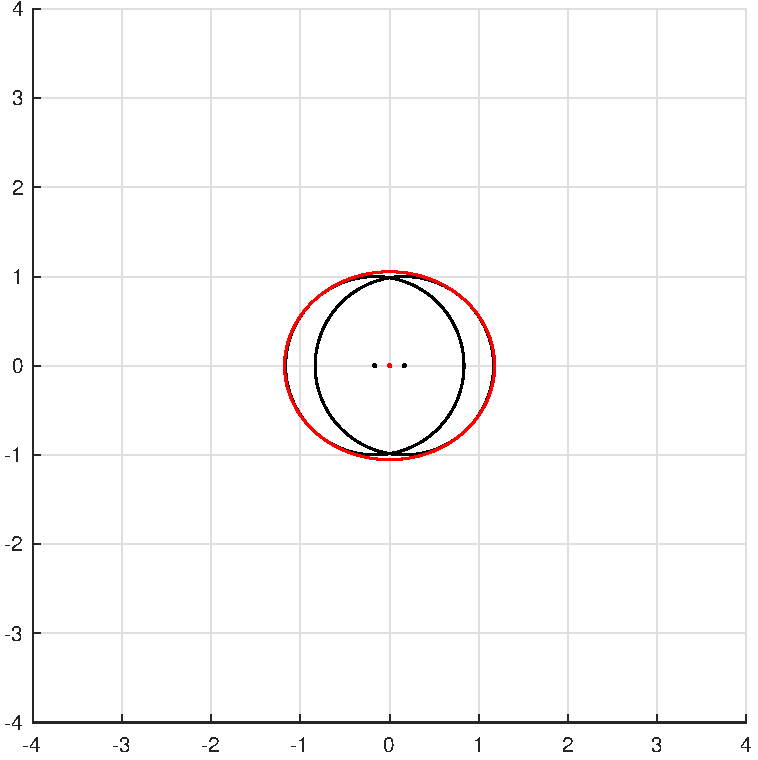
\includegraphics[width=0.3\textwidth]{union_offset_oa/7.pdf} & 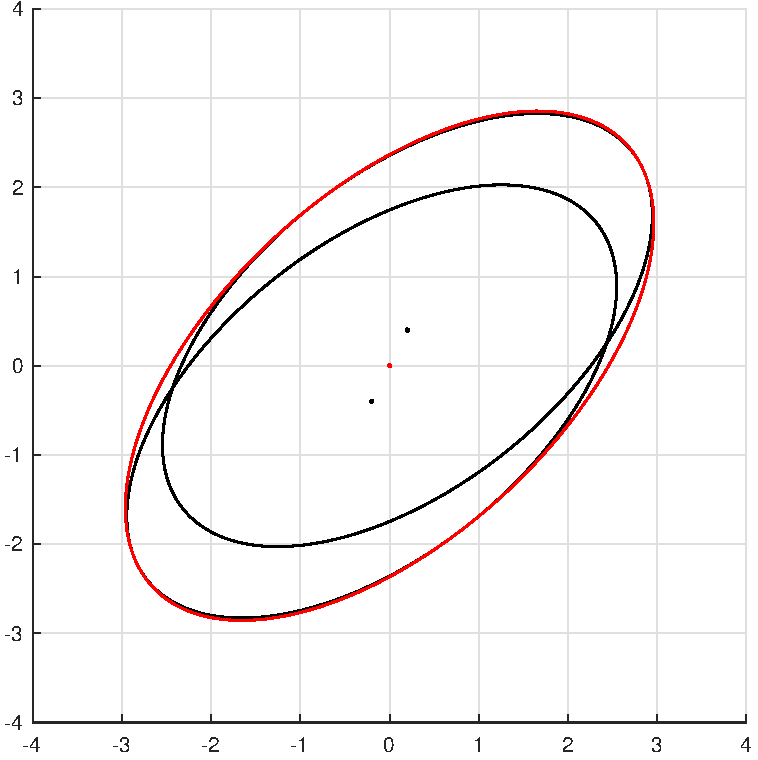
\includegraphics[width=0.3\textwidth]{union_offset_oa/8.pdf}\\
		Offset by $2v_2$ & \makecell{Apply an affine transformation \\such that the ellipsoids \\become unit spheres} & Affine transformation back
	\end{tabular}
	%\caption{Table of figures}
	\label{union_offset_oa2}
\end{table}

\textcolor{red}{TODO: prove that this algorithm gives the minimum outer approximation. }

The implementation is in \texttt{ellipsoidal\_approximation/union\_offset\_oa.m}


\subsection{Minkowski sum of an ellipsoid and a parallelotope, inner approximation}
Using the same idea in section \ref{intersect_offset_ia}. However, this approximation is not optimal. \textcolor{red}{TODO: find the closed-form optimal approximation.}

\begin{table}[h!]
	\centering
	\begin{tabular}{ccc}
		\includegraphics[width=0.3\textwidth]{union_offset_ia/1.pdf} & \includegraphics[width=0.3\textwidth]{union_offset_ia/2.pdf} & 
		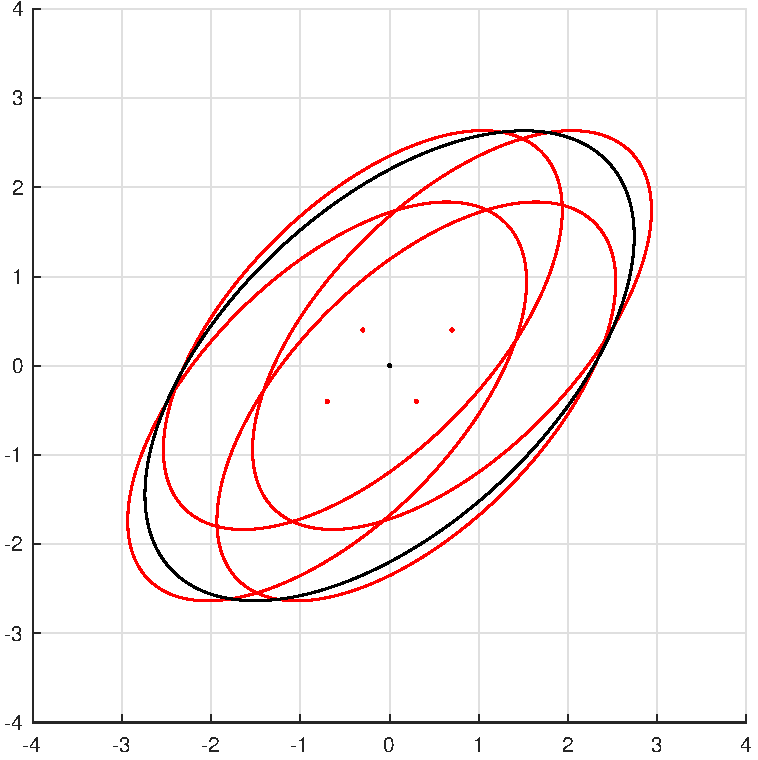
\includegraphics[width=0.3\textwidth]{union_offset_ia/9.pdf}\\
		\makecell{Ellipsoid and parallelotope. \\ The two arrows are the control \\ vectors that form the parallelotopic \\ control set.}& \makecell{Red ellipsoids are obtained by \\ shifting the blue ellipsoid to each \\ vertex of the parallelotope.\\ The Minkowski sum is \\the convex hull of red ellipsoids.} & \makecell{The black ellipsoid is the\\ calculated inner approximation.}
	\end{tabular}
	%\caption{Table of figures}
	\label{union_offset_ia1}
\end{table}

\begin{table}[H]
	\centering
	\begin{tabular}{ccc}
		\includegraphics[width=0.3\textwidth]{union_offset_ia/3.pdf} & 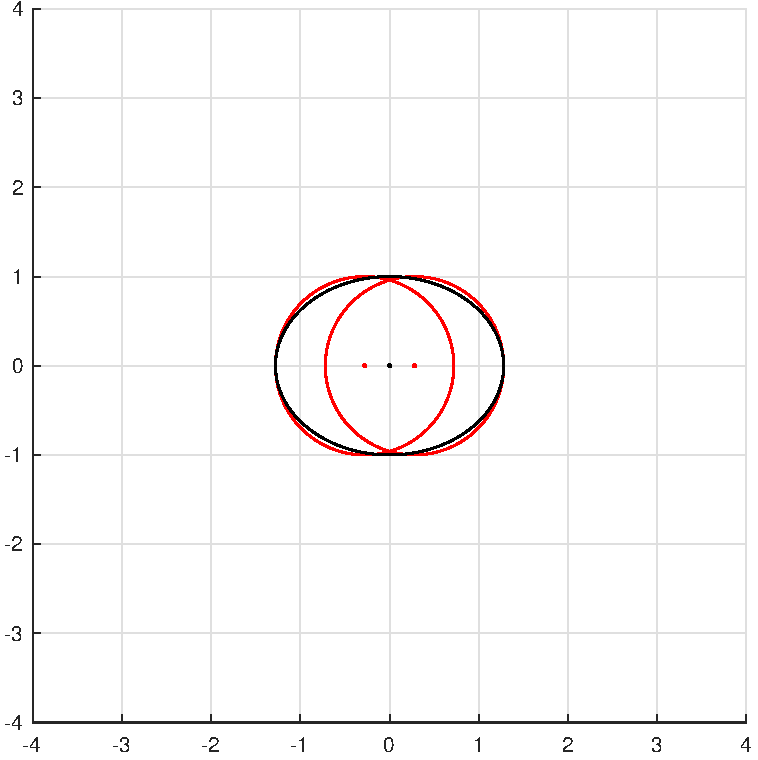
\includegraphics[width=0.3\textwidth]{union_offset_ia/4.pdf} & 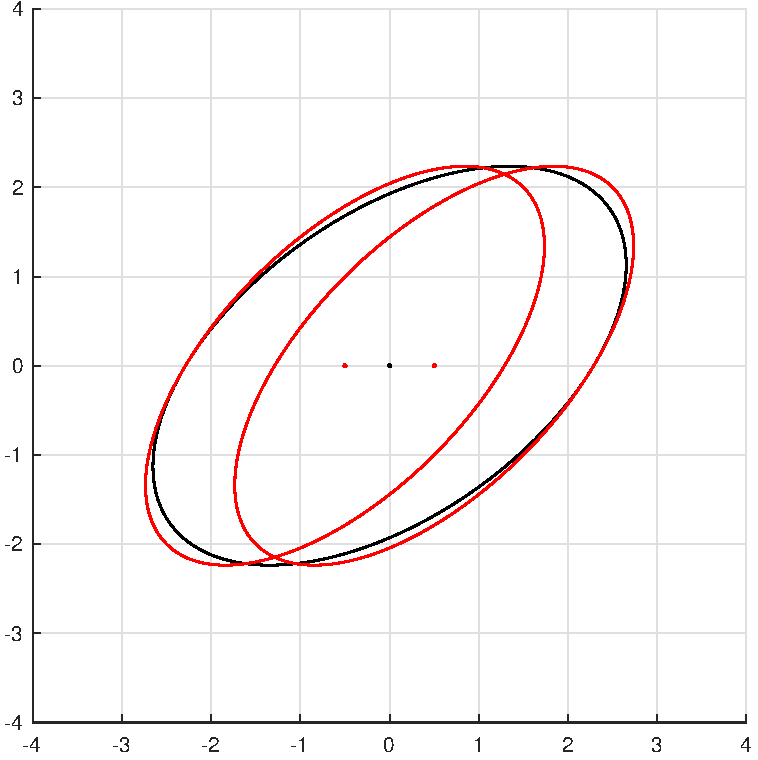
\includegraphics[width=0.3\textwidth]{union_offset_ia/5.pdf}\\
		Offset by $2v_1$ & \makecell{Apply an affine transformation \\such that the ellipsoids \\become unit spheres} & Affine transformation back \\
		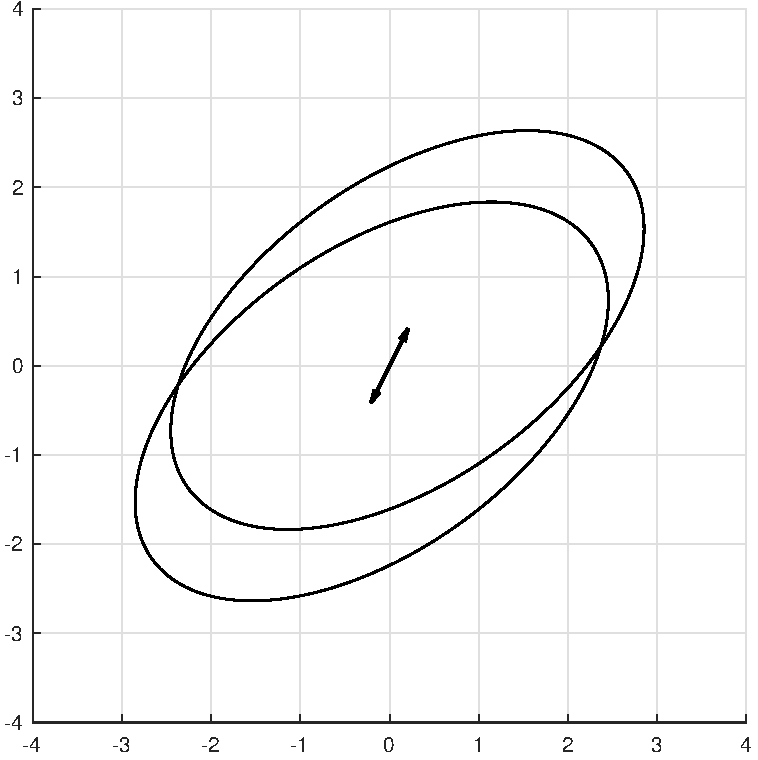
\includegraphics[width=0.3\textwidth]{union_offset_ia/6.pdf} & 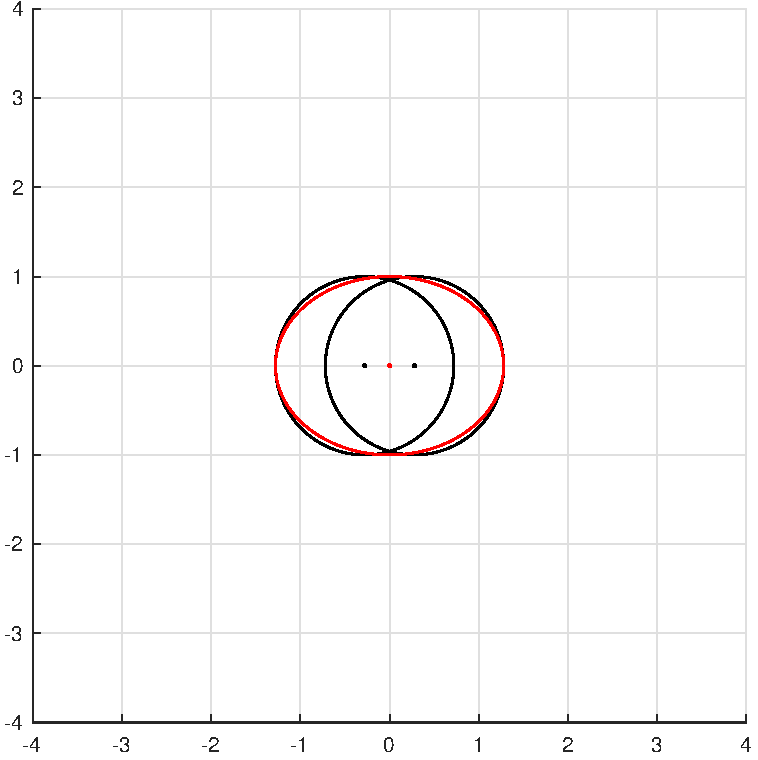
\includegraphics[width=0.3\textwidth]{union_offset_ia/7.pdf} & 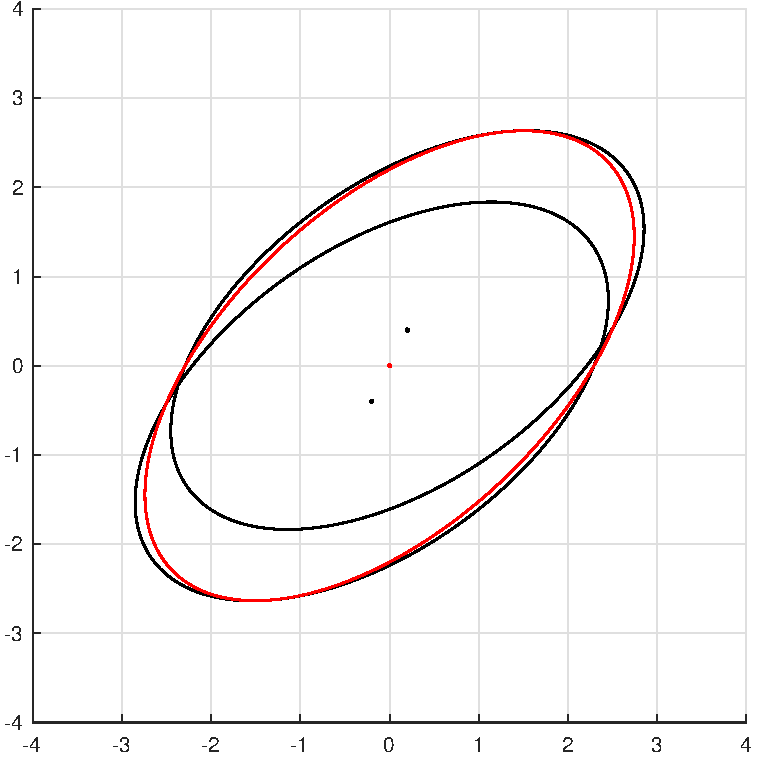
\includegraphics[width=0.3\textwidth]{union_offset_ia/8.pdf}\\
		Offset by $2v_2$ & \makecell{Apply an affine transformation \\such that the ellipsoids \\become unit spheres} & Affine transformation back
	\end{tabular}
	%\caption{Table of figures}
	\label{union_offset_ia2}
\end{table}

The implementation is in \texttt{ellipsoidal\_approximation/union\_offset\_ia.m}

\subsection{Minkowski sum and difference of two concentric ellipsoids}
Since I didn't use ellipsoids to approximate the set of control/disturbances, this section is just for future reference, and the derivation is from [2] section 2.2 and section 2.3.

The implementation is in the following files.
\begin{table}[h!]
	\centering
	\begin{tabular}{|c|c|}
		\hline
		Minkowski sum outer approximation& \texttt{ellipsoidal\_approximation/minksum\_ellipsoid\_oa.m} \\
		Minkowski sum inner approximation& \texttt{ellipsoidal\_approximation/minksum\_ellipsoid\_ia.m} \\
		Minkowski difference outer approximation& \texttt{ellipsoidal\_approximation/minkdiff\_ellipsoid\_oa.m} \\
		Minkowski difference outer approximation& \texttt{ellipsoidal\_approximation/minkdiff\_ellipsoid\_ia.m} \\
		\hline
	\end{tabular}
	%\caption{Table of figures}
	\label{minksum_diff_ellipsoids}
\end{table}

These methods can only be applied to the case where the two ellipsoid has the same dimension, and it is not clear if the method can be applied to degenerated ellipsoids.

I am not sure if there are cases where the set of control is ellipsoid. Also, the dimension of control could be less than the dimension of states, but these methods require the dimensions are matched.

However, it might be useful to model the set of unmeasurable disturbance as an ellipsoid if they are close to Gaussian noises.

\begin{thebibliography}{9}

\bibitem{ellipsoid-toolbox}
Kurzhanskiy, Alex A., and Pravin Varaiya.
Ellipsoidal toolbox (ET).
Proceedings of the 45th IEEE Conference on Decision and Control. IEEE, 2006.

\bibitem{ellipsoidal-calculus}
Kurzhanskiĭ, A. B., and István Vályi. Ellipsoidal calculus for estimation and control. Nelson Thornes, 1997.

\bibitem{control-tube}
Kurzhanski, Alexander B. "Dynamics and control of trajectory tubes. Theory and computation." 2014 20th International Workshop on Beam Dynamics and Optimization (BDO). IEEE, 2014.

\bibitem{convexopti}
Boyd, Stephen, and Lieven Vandenberghe. Convex optimization. Cambridge university press, 2004.

\end{thebibliography}
\end{document}
